   % !TEX TS?program = pdflatexmk
                    \documentclass[a4paper, 12pt]{article}
                  \usepackage[english]{babel}
                  \usepackage[utf8]{inputenc}
    		\usepackage[utf8]{inputenc}
    %                \renewcommand{\baselinestretch}{1.0} 
                    
                    
                    %MARGINS
                    \usepackage[left=25.4mm, right = 25.4mm, top=25.4mm, bottom=25.4mm, includefoot]{geometry}
      %            \geometry{a4paper, total={170mm,257mm}, left=25.4mm, right = 25.4mm, top=25.4mm, bottom=25.4mm}
                    \setlength{\parindent}{0in}
                    \usepackage{enumitem}
                   
                    %Adding pictures
                    \usepackage{graphicx}
                    \usepackage{float}
                    
                    %Header and footers
                    \usepackage{fancyhdr}
                    \pagestyle{fancy}
%                    \fancyhead{}
                    \fancyfoot{}
                    \fancyfoot[R]{ \thepage\ }
                    \renewcommand{\headrulewidth}{0pt} %change the pt width to insert header line
                    \renewcommand{\footrulewidth}{0pt} %change the pt width to insert footer line
                    \usepackage{amsmath}
                    \fancyhf{}
                    
%    	\rhead{\leftmark}
%    	\lhead{Guides and tutorials}
	\rfoot{Centre for Civil Society \hspace{1mm} \textbar \hspace{1mm} www.ccs.in \hspace{2mm}  \thepage}
%             \lfoot{  \leftmark }     			% get the section heading on the footer 
                   
                   
                    %Tables
                    \usepackage{longtable}
                    \usepackage{booktabs}
                    \usepackage{subfig}
                    \captionsetup{aboveskip=14pt,}
                    
                    %Coloured Boxes
                    \usepackage{xcolor}
                    \usepackage{mdframed}
                    
                    %Custom Spacing
                    \usepackage{setspace}
                    
                    %Defining Colours
             \definecolor{CCSbrown}{RGB}{163, 86, 37}
               \definecolor{CCSblack}{RGB}{167, 169, 172}
                 \definecolor{CCSblack}{RGB}{64, 64, 65} 
             
             
             %Heading colours                  
                    \usepackage{sectsty}
                    \usepackage{titlesec}
    		\chapterfont{\color{blue}}  % sets colour of chapters font
    		\sectionfont{\color{CCSbrown}}  %sets colour of section font
    		\subsectionfont{\color{CCSblack}} %sets colour of subsection font
    		\subsubsectionfont{\color{CCSblack}} %sets colour of subsubsection font
    		
		
		%Bibliography
		
		\usepackage[authordate, backend=biber]{biblatex-chicago}
		\addbibresource{bibliography5.bib}
\usepackage{hyperref}
		\hypersetup{
colorlinks,
linkcolor=black
citecolor=CCSbrown,
urlcolor=black}
\usepackage{blindtext}

                    \begin{document}
                    
    %==================================================                
                    %TITLE PAGE
                    \begin{titlepage}
                    	\begin{center}
                    	\line(1,0){300}\\
                    	[0.25in]
                    	\huge{\bfseries \textcolor{CCSbrown} {Disruption on Demand}} \\
    	[0.5cm]
    	\large  {A Study of How Aggregators are Challenging \\ the Regulatory Structure} \\
    	
                    	\line(1,0){200}\\
                    	[1in]
                    	\textsc{\big Jayana Bedi, Adarsh Ranjan \\ Jibin Joseph, Prajwal Seth} \\
                    	[1.5cm]
                    	{\Large September 2018} \\
                    	[2.0cm]
    %    	{\huge Researching Reality Internship 2018} \\
     %   	[0.5cm]
                    	{\LARGE Centre for Civil Society} \\
                    	[0.1mm]
                    	{\Large New Delhi, India} \\
    	[2.0cm]
    	 
\includegraphics[width = 75mm]{CCSlogo.jpg}
      
                    	\end{center}
                    \end{titlepage}
     %=====================TOC===============================================                 
                    \tableofcontents
                    
      
                    
                    %EXECUTIVE SUMMARY
                    \newpage
                    \section*{Executive Summary}
                    \addcontentsline{toc}{section}{Executive Summary}
                   Aggregators in India are riddled with uncertainty and suspicion. Since they play the role of technology mediators and not 'service providers', they are able to claim exemption from regulations. Regulators who aim to guarantee consumer protection face the conundrum of how to manage aggregators in the marketplace. Their definition and treatment and the liabilities that ought to be imposed on them are all unclear. Since aggregators provide a platform for several, small, individual entrepreneurs to access the marketplace, redrawing the regulatory framework for these service industries without throttling entrepreneurship or opportunities for self-employment is a non-trivial challenge. \\
                    
                    Our study on aggregators in India comes in response to the debate around the way in which aggregators ought to be regulated. By focussing on four aggregators, Airbnb, Uber, UrbanClap and Zomato \footnote{While Airbnb and Uber are foreign companies (headquartered in San Francisco) that have extended their market to India through their Indian subsidiaries, UrbanClap and Zomato are of Indian origin.}, we argue that understanding how they inadvertently tackle questions of consumer protection can help in redrawing the regulatory frameworks. \\
                    
                   First, we highlight the consumer protection challenge being tackled by aggregators through an analysis of some of the mechanisms they put in place, especially those that increase information exchange between consumers and enable a collective governance framework on the platform. We argue that trust mechanisms employed by aggregators in India act as proxies for service standards by analysing three such mechanisms: post-service feedback, checks against dishonest behaviour and monitoring safety and quality standards. We find that while fake and biased ratings are a serious threat to the credibility of online reputation mechanisms, aggregators are taking several corrective measures to stem them. We also highlight the important role played by insurance in the way aggregators deal with broken trust.\\
                    
                  In the next section, we contrast the existing regulations with the service standards that aggregators put in place for the same service. We study regulations in the two services where aggregators have caused considerable disruption, hospitality and taxicabs. Using data mining, we create a comprehensive database of listings on Airbnb in Delhi and carry out a sentiment analysis of the reviews to highlight how, in many instances, the needs of the consumers are at odds with what regulations deem important. In the case of taxi regulations, we highlight how certain conditions put in place by the regulations are difficult to implement and have limited enforceability. In both these service industries, we find that existing prescriptive rules increase the regulatory burden on enterprises but fail to meet the key goal of consumer protection as state capacity is thinly spread. We find that the ex-post measures of quality assurance employed by online platforms, such as Airbnb and Uber, are better suited to reflect the dynamism of the market. These aggregators replace prescriptive norms with information, incentives and strong feedback mechanisms.    \\
                    
                 Finally, we argue that the aggregators' approach of prizing trust and diversity are fast rendering certain traditional regulations obsolete and showing the way for a principle-based approach. State capacity can be relieved by replacing prescriptive specifications with the mechanisms of trust creation employed by aggregators and potentially imposing liabilities on aggregators that meet the good-faith standards of consumer protection. \\

        
                    
                    %INTRODUCTION
            
                    \section{Introduction}
                 Regulations in India, which aim to protect consumer interests by ensuring fair trade and correcting information asymmetries \parencite{Dudely, Brito 2012, 11-14}, are typically product based and reactionary and thereby restrain innovation. In addition, due to the tendency of regulatory capture by traditional players, the regulatory intent of protecting the consumers is rarely met while the costs of entry and operation for enterprises remain high.. \\
                    
                   Over the last decade, particularly in the services sector, technology has changed the game. Enterprises that provide a low-cost platform to connect service providers and customers have mushroomed. Aggregators like Airbnb, Uber and Zomato have stepped in to meet rapidly escalating and changing consumer demands. \\
                   
                   Aggregators that offer services such as ridesharing and peer-to-peer accommodation are growing at rates much higher than their traditional counterparts are. For instance, Uber in India has claimed that its business is growing over 100\% year on year, due to the adoption of services like pool and expansion into smaller cities \parencite{PTI2017}. ). It has over 3 lakh drivers and manages to complete over 10 million weekly trips \parencite{PTI2018}. Similarly, Airbnb has made major inroads into India with nearly 200\% growth in 2016 to 2017 \parencite{Laghate 2017}. Some of the reasons for aggregators having seen such a rapid growth include their ability to reduce the cost of market entry and to achieve greater operational efficiency. \\ 
                    
                  Their rapid growth has raised public debate on the nature of regulations and the responsibilities that these aggregators must bear. In India, aggregators operate in a regulatory vacuum due to a lack of clarity on their definition. At the heart of the discussion on what rules ought to govern aggregators is the question of whether they are trying or will try hard enough to protect the interests of consumers.\\

                   While increasing the size of the market, aggregators have inadvertently begun tackling questions of consumer protection and information asymmetry.\\
                     
                     The business model of online platforms is to meet user expectations by reducing the information asymmetries through crowd-sourcing and making information on past transactions inexpensive and transparent. Leveraging technological developments, aggregators coordinate dispersed knowledge about buyers and sellers to facilitate transactions\parencite{thierer2015internet}. \\
                    
                    Using feedback and reputational mechanisms that allow for reviewing both the quality of the product and the trustworthiness of the seller, aggregators are developing new ways to mitigate the vulnerabilities and risks involved in carrying out a transaction. In addition, by instituting ‘community standards’, they are gradually building monitoring capability to protect the interests of the consumers. Even in the absence of complete information on both sides (buyers and sellers), the series of incentives and disincentives put in place by aggregators encourage ‘bad’ actors to be weeded out from the platform. \\
                    
                  Given the volume of transactions on these online platforms, the benefits from this collective governance model accrue to individuals even outside of such interactions. Scholars argue that besides enabling optimal resource allocation \parencite{Hamari et al., 2015}, the sharing and on-demand economies will promote safety and effectiveness \parencite{Feeney et al. 2015; Lee et al. 2008}, improve human development \parencite{Hancock 2001}, create more jobs \parencite{Fang et al. 2015}, rationalise the use of energy \parencite{Kriston et al. 2010; Belk 2014; Martin et al. 2011; Rifkin 2015; Leismann et al. 2013}, and reduce greenhouse gas emissions \parencite{Martin et al. 2011; Costain et al. 2012; Steininger et al. 1996}.\\

                   
                    
                    %Consumer Protection Through Trust Mechanisms in the Aggregator Business Model
                    \section{Consumer Protection Through Trust Mechanisms in the Aggregator Business Model}
                    
                    Market participants in any economy recognise that each one of them is keen on maximising their self-interests. Hence, before any transaction, they are likely to view the transacting party with mistrust.\\
                    
                    One way in which markets have responded to this challenge is through the price system, which is based on the valuation of goods by consumers. An offline marketplace has many other mechanisms to establish trust, including seeking referrals, viewing credentials, participating in service trials, consultations, using guarantees, warranty or trusting a middleman \parencite{thierer2015internet}.\\
                    
                  A lack of trust that enterprises will serve consumer interests also creates public demand for governmental intervention in the form of ex-ante regulations. In particular, countries with lower levels of trust and high corruption see greater demand for interventions in the form of regulations \parencite{aghionpaper}. In addition, excessive regulation may discourage the formation of trust \parencite{aghionpaper}. In such a scenario, trust mechanisms play an important role in complementing or acting as a substitute for formal enforcement mechanisms \parencite{thierer2015internet}. \\
                    
                    In India, the emergence of aggregators in sectors such as hospitality (Airbnb), taxi services (Uber and Ola) and food (Swiggy and Zomato) has led to the development of new trust-building mechanisms and the integration of existing ones within these platforms. In this section, we have consolidated the various methods aggregators use to build trust between the users based on an analysis of their websites and interviews with aggregators and their service partners. These include reputation and feedback mechanisms, checks against dishonest behaviour, and monitoring safety and quality. We discuss the susceptibility of feedback mechanisms to fraud and the measures aggregators use to check these in order to maintain trust. Finally, we discuss ways in which aggregators deal with broken trust in the form of insurances and grievance redressal.\\
                    
                    \subsection{Trust Mechanisms Employed on Platforms }
\subsubsection{Collecting Customer Feedback Through Ratings and Reviews}
                    
          Platforms have used buyer incentives to gather maximum information about products and services as an entrepreneurial opportunity, developing robust reputational and feedback mechanisms \parencite{thierer2015internet}. The mechanisms usually involve the supplier and the consumer giving each other an overall rating or specific ratings based on certain parameters. Ratings may also be accompanied by a written review, providing future buyers and sellers with useful information about the transaction. Reviews serve as guiding points, discouraging or encouraging exchange between individuals. By making information about the product and the seller easy to find, widely available and inexpensive, these reputational feedback mechanisms have lowered transaction costs \parencite{EYreport}.\\

\subsubsection{Information Made Easy Through the Aggregation and Organisation of Feedback}
                    
                    While each individual’s evaluation of a transaction differs based on their perception of quality, the systematic organisation and categorisation of the reviews and ratings help provide a fair assessment of a seller or buyer. Aggregators follow different approaches to ensure that the most useful information is communicated in the right way. \\
                    
                    For example, Airbnb provides a breakdown of ratings on parameters such as accuracy, communication, location, cleanliness, check-in and value. Further, while viewing listings in other countries, a user is first shown the reviews written by people from his country. By being sensitive to the idea that an individual’s needs and expectations are shaped by their cultural and social contexts and likely to be anticipated or recorded by their compatriots, Airbnb enhances the experience for users. \\

Similarly, while calculating average rating of a restaurant, Zomato allocates higher weightage to ratings given by top-rated reviewers. It also displays such users’ reviews before others. This increases trust on the platform by ensuring that reviews considered useful by people are discovered first \parencite{GoyalD2012}. \\
                    
                    \subsubsection{Evolving Feedback Tools}
                    
                   In order to stay dynamic, effective and responsive to evolving consumer needs, aggregators constantly adjust their feedback tools. For example, Zomato introduced hygiene ratings for restaurants in collaboration with third-party hygiene auditors. This was motivated by a survey conducted by Zomato where 93\% of platform users gave more weightage to restaurant hygiene than factors such as the taste of food \parencite{GoyalD2017}. Figure 1 and Figure 2 provide a breakdown of the hygiene parameters on which restaurants were graded. However, Zomato recently removed this breakdown and chose to only display the overall hygiene rating. \\

\includegraphics[height = 4.3in]{fig1 and fi2.png}

	\subsubsection{Using Customer Feedback to Ease Market Entry and Reward Good Behaviour}
                    
 Feedback systems based on reputation provide novel ways for new service providers to come up to par with those already existing on the platform. UrbanClap, for instance, asks past customers or colleagues to write references for a new service provider on the platform. Airbnb too allows hosts and guests to receive public references from friends, family members and colleagues to help build their profile. This enables transferring the trust built in one context to another, relatively unfamiliar context and eases entry on the platform.\\
                    
                 Ratings also enable users to collectively reward trustworthy behaviour with increased business. Some platforms actively ensure that trustworthy sellers receive a competitive advantage. The ‘superhost’ status awarded to reliable and highly rated hosts on Airbnb is one example of this \footnote{The ‘superhost’ status is accorded to hosts who have a rating above 4.8, a response rate above 90\%, received at least 10 bookings in a year, and initiated 0 cancellations.}.  Superhosts earn 22\% more than other hosts on an average, receive priority support during grievance redressal and enjoy increased visibility on the platform.\footnote{Other benefits include additional referral bonus, travel vouchers and special superhost discounts.}   \\

Further, the personal profiles of users serve as ‘social cues’ or ‘trust signals’ and facilitate decision-making. A study by Eyal Ert, Aliza Fleischer and Nathan Magen reveals how the perceived trustworthiness of a host based on their personal photo increases or decreases the probability of transacting with them \parencite{ert2016trust}.\\

The UrbanClap partner app displays the top six, most highly rated professionals in each category to all professionals to encourage the trustworthy behaviour. \\

Since positive reputation acts in favour of service providers, it becomes ‘rational’ or ‘profitable’ for them to be trustworthy. In this way, ratings and reviews constantly keep service quality in check and increase their likelihood of meeting consumer expectations.\\

                    
                    \subsubsection{Minimising Distortions and Biases in Ratings and Reviews}
                    
                    According to the Local Consumer Review Survey by BrightLocal in the USA, 54\% of consumers consider the average star rating to be the most critical factor. Eighty-four percent of the respondents trusted online reviews as much as a personal recommendation and 91\% of the respondents read reviews to determine if a local business is good or bad (BrightLocal 2017). \\ 

Ensuring that reviews remain representative of service quality and consumer experience is no mean challenge. Not all reviews are equally informative, and it can be tedious and time-consuming for a consumer to go through each review. In addition, fake reviews could also abound. Recent studies have also revealed that 15\% to 30\% of all online reviews are false \parencite{ivanova2017can}. In India, platforms such as Zomato that allow users who have not transacted to give feedback may create situations where sellers write positive reviews for themselves and negative reviews for their competitors. Reviewers on these platforms may solicit meals in exchange for good reviews, raising questions on the authenticity of a review \parencite{ChaddahP}.\\

Consumers typically respond more to the coarser information provided by average ratings than reviews \parencite{dai2012optimal}. Ratiholengs, however, could be hostage to selection biases: first, only consumers with an expected positive utility will purchase the product in the first place, giving rise to an acquisition bias; and second, even within the people who bought the product, only consumers with distinctly positive or negative experiences are likely to provide feedback, leading to an over-representation of these experiences in the sample of reviews. A study of ratings on Amazon reveals that they exhibit a bimodal distribution with more positive than negative reviews \parencite{luca2016fake}. An analysis by Hu, Pavlou and Zhang \parencite{hu2017self}  shows that consumers are not entirely rational and are unable to adjust for the effect of these biases, making rating an inaccurate proxy for the product. Bhole and Hanna (2017), on the other hand, find that, in fact, the underreporting bias does not decrease the effectiveness of the mean star rating except for in cases where the product quality is either extremely high or low.\\

Aggregators try to mitigate these risks using a few methods.\\

An over-representation of people with extreme experiences can be solved either by providing incentives to encourage all users to review or by making rating compulsory for every transaction. Some aggregators offer monetary incentives (in the form of discounts or coupons) while others like Glassdoor follow a give-to-get policy. Ola, a taxi aggregator in India, requires a user to rate the previous ride before they can book the next one, ensuring the evaluation of every trip and not only very good or bad ones. However, in Uber, a user can skip the option to rate. On Airbnb, well over 75\% of stays end in a review, and this has become one of their signature features.\footnote { Written evidence from Airbnb’. Last modified December 2015. https://bit.ly/2MUOXEC} \\

To remedy the errors associated with fake ratings, Zomato ranks every rating to give higher weightage to trustworthy entries and removes dubious entries from the calculation while generating the mean rating of a restaurant (Goyal 2012). It has also introduced a system—similar to the one suggested by Luca \parencite{luca2016reviews}—that uses algorithms to mine text and characteristics giving specific reviews more weightage than to others. Reviews identified as a trustworthy feature at the top of a restaurants’ page. \\

The challenge of fake or promotional entries is lower for platforms like Uber and Airbnb where a user can only rate and review after a transaction has occurred.\\ 

                                   
                    \subsection{Checks Against Dishonest Behaviour}
                    
                   Besides the use of ratings and reviews to deter dishonest behaviour, aggregators also put in place additional checks to prevent suspicious activities. \\

For instance, Airbnb claims to use predictive analytics and machine-learning algorithms to assess the risk score of every booking and to identify and investigate suspicious activities before they happen. Irrespective of the validity or rigour of their approach, they use other means to penalise bad behaviour. For example, hosts who cancel confirmed reservations have an automated review posted on their profile as a penalty for cancellation. Airbnb also does not allow a user to review a guest or a host unless the stay actually happened. Additionally, in 2014, their system was updated to create a process of ‘double blind’ reviews, where neither side gets to see the review before it is published to allow for candid, honest and unbiased feedback.  \\
                    
                  Uber tracks the activities of drivers and may deactivate their account in case of excessive cancellations, a deliberate increase in the time or distance of a trip, an acceptance of trips without the intention to complete them, claiming fraudulent charges or creating dummy driver accounts for fraudulent purposes. They also claim to deactivate the account permanently if a routine motor vehicle record or background check reveals anything that violates Uber safety standards (or any other criteria depending on local regulations). \\

The content team of Zomato regularly verifies the menu, timings and other details of each restaurant to ensure that only genuine restaurants are listed on the platform. Furthermore, following growing incidents of spam, fake and plagiarised reviews, Zomato rolled out a rule in 2017 to limit the maximum number of reviews by an individual to 10 per month \parencite{Narang17}. \\

Finally, UrbanClap discourages dishonest behaviour by publishing a list of ‘blacklisted professionals’ on its website \footnote{‘Blacklisted Professionals’. UrbanClap. Accessed 17 July 2018. https://bit.ly/2OI73vv}  to protect customer interest. \\
                    
                    \subsection{Establishing Identity for Quality and Safety }
                    
                    In order to build credibility and increase trust in their brand, aggregators monitor the quality and safety of the platform. They set a minimum threshold of ratings that suppliers, and often consumers, must meet to continue operating on the platform. Table 2 highlights the importance accorded to higher ratings, with more than 90\% of the listings having a rating of 4.5 stars or above (on a 5-star scale). \\

Aggregators carry out the verification of government identity documents (IDs) and licences to establish the identity of users. Uber and UrbanClap make it mandatory for partners and service providers to provide specified government IDs. Airbnb also collects the government IDs (driver’s licence, passport, visa, etc.) of hosts and guests. Similarly, Zomato now collects the Food Safety and Standards Authority of India licence of restaurants before listing them. These measures deter fake profiles on the platform.\\

These aggregators increase safety by providing details of not only the service/product but also the transacting individuals. Uber, for instance, allows riders to view the detailed profile of their driver, including compliments that other riders have given and milestones achieved by the driver. The riders can find safety tips built in partnership with law enforcement and obtain details of the driver screening processes, insurance protections and community guidelines. Uber also allows both riders and drivers to share their location with up to five people while on a trip. \\

In the case of Airbnb, guests and hosts are encouraged to link their online identities—Facebook, Twitter and LinkedIn—with their Airbnb profiles. This provides insight into people’s personalities and interests and increases the chances of people representing themselves accurately. Further, it allows guests to send their prospective host a message (with the host having the discretion to accept or decline) in a bid to increase familiarity. \\

               
                    
                    \subsection{Actions Taken When Trust Is Broken}
                    
                    Although the trust mechanisms employed by aggregators provide a layer of protection to consumers, trust and safety are also contingent on the dispute resolution and grievance redressal facilities available when trust is broken. The aggregator model of business introduced distributed trust \parencite{BotsmanR}. Since trust becomes distributed across people interacting on the platform and between the platform and the people, so does accountability.\\

While aggregators expand opportunities for consumers and service providers, they also increase the risks of sharing resources. Demarcating obligations and laying down where the onus lies in case trust is broken has always been a point of contention in the aggregator business model. To avoid this from constraining their growth prospects, aggregators often insure users against any plausible damages. A survey conducted by Lloyd revealed that the 71\% of consumers (out of a sample of 5,000) globally would be more comfortable using sharing economy services if insurance was offered and 70\% were more likely to consider sharing or offering a service if insurance was offered. \\

It is in this context that we see the emergence of insurance programs, such as the Host Guarantee Program by Airbnb, which covers hosts for damages of up to Rs. 6,00,00,000 caused by a residing guest. The host has to first contact the guest and try to settle the claim with them. If this fails, the host must review Airbnb's Host guarantee terms and determine their case’s eligibility \footnote {Hosts are advised to file a police report, and this is mandatory in case the claim amount exceeds \$300 (approximately Rs. 20,700). After doing so, the host must submit all relevant. documentation to Airbnb via a web form. The request has to be filed within 14 days of the dispute or before the next guest checks in, whichever is earlier.}.  Following this, Airbnb analyses the documentation and gives a decision on the claim. \\

Similarly, treating its driver partners also as customers on the platform, Uber rolled out free insurance for more than 4,50,000 drivers on its platform in India, as a part of its remuneration deal for them. This insurance policy announced by Uber in 2017, through collaboration with ICICI Lombard General Insurance Co., includes accidental death, disablement, hospitalisation and medical treatment. \footnote{The program includes as much as Rs. 500,000 for death insurance, Rs. 500,000 for permanent disability and Rs. 200,000 for hospitalisation coverage.}  Uber and other rideshare aggregators in India are also experimenting with per ride insurance options for passengers, along the lines of air travel (Venkatesh 2017). \\
                    
                    UrbanClap also provides insurance up to Rs. 10,000 to customers for damages done by a professional while delivering services. \\

Lastly, aggregators make use of customer care helplines and chat support systems for addressing grievances. Using these, both customers and service providers on Airbnb, Uber and UrbanClap can report issues. Airbnb also has an urgent customer support helpline number for travellers to report physical harm. Uber allows drivers to avail help and registers complaints through a designated 24 x 7 customer service helpline.\footnote{These include instances of where the driver was unprofessional or if the driver’s face did not match.}  In case, a user rates an Uber trip four stars or below, the app allows the user to give reasons why they believe that the service was of inadequate quality. \footnote{The app provides multiple options that the user can select for easy access. These include, but are not limited to, price, professionalism, comfort, driving, music and route taken. }.  Uber considers this feedback while monitoring the behaviour of drivers in the future. It can subsequently block the Uber partners account until they visit an Uber greenlight hub and resolve the dispute.\footnote{Grievance redressal cells for drivers are located at several locations in the city.}  With the help of these insurance programs and helpline numbers, aggregators are taking greater accountability in dealing with broken trust.\\

                    \section{Limitations of the Current ‘Specification-Centric’ Regulatory Framework in \\Accommodating Aggregators}
In India, regulations tend to be overly prescriptive or entirely proscriptive, and state capacity for enforcement is limited. The differences between traditional suppliers and aggregators make it impractical to co-opt existing regulations. Furthermore, most government directives tend to establish uniform service specifications across industry participants, restricting not only supplier entry but also access for consumers who do not necessarily seek the same level of quality. As opposed to uniform service specifications, aggregators rely on the power of information and trust mechanisms to enable the community to decide and regulate. The persistence of uniform service specifications, whose initial justification is no longer valid, not only imposes costs on businesses but may also work against the interests of consumers \parencite{koopman2014sharing}. \\  

In this section, we contrast government regulations with comparable mechanisms employed by aggregators that seek to protect the interests of consumers. We look at the two sectors—bed and breakfasts (B\&Bs) and taxi providers—that have grabbed attention as disruptors of traditional markets and, consequently, many demand greater regulation and scrutiny of their operations. For B\&Bs, we evaluate how the mechanisms adopted by them manage to meet consumer expectations of quality. Using the text mining software Leximancer, we mined reviews of all Airbnb listings in Delhi. An analysis of these reviews provides a list of the most commonly occurring words in the reviews, revealing the amenities that are most important for guests. For the section on taxis, we examine the conditions laid down by the City Taxi Scheme 2015 and the requirements under Uber that expand opportunities for service providers while, at the same time, protect the interests of consumers.\\                   
                    
           
                    \subsection{Contrasting Regulations Governing Bed and Breakfasts with Mechanisms Used by Airbnb}

A B\&B is a small, independent establishment for overnight accommodation and breakfast. In Delhi, a B\&B is not treated as a commercial unit and one does not require a licence to provide food or lodging services to the guests (Chapter 3, point 15). Any family may voluntarily choose to register itself either under the National Capital Territory of Delhi (Incredible India) Bed and Breakfast Establishments (Registration and Regulation) Act 2007 or under the ‘The Incredible India Bed and Breakfast Establishments Scheme’ of Government of India.\footnote{An establishment registered with the latter is automatically approved and registered under the former.}  The objective of the two schemes is to ‘provide a clean and affordable place for foreigners and domestic tourists alike including an opportunity for foreign tourists to stay with an Indian family to experience Indian customs and traditions and relish authentic Indian cuisine’ (Source). \\
                    
  Registration under The Delhi Bread and Breakfast Establishment Act imposes certain restrictions on the owners of such properties. The owner is required to: 
\begin{itemize}
\item Physically reside in the property;
\item Maintain a register or computerised record in electronic form, giving detailed particulars of the guests, and keep it available for inspection at all times;
\item  Send information about the guests staying in the establishment to the local authority and the police every fortnight on the 15th and last day of every month;
\item Not maintain a front office and the entire house should appear like a normal residential house;
\item Not carry out or allow any commercial activity of tours and travel, sightseeing, transport, handicrafts or any other similar activity in or from the establishment;
\item  Not allow guests to run a separate kitchen in the establishment.
\end{itemize}                                  
Besides these, the checklist for approval and registration lays out specific requirements to categorise units as silver or gold. There are 36 requirements in total. We discuss some of these and contrast them with the approach followed by Airbnb.\\

	\subsubsection{Specific Requirements Versus Disclosure Norms}
The Act defines a room as ‘a bedroom with not more than two beds and provision for extra beds for children accompanying the guest’. A silver category B\&B must have a room of 20 sq. ft. whereas gold must have a room of 200 sq. ft. . In contrast, Airbnb does not impose any restrictions on the size of the room or the number of beds in it.\\

The Act mandates each room have an attached bathroom with 24-hour running hot and cold water. It specifies the size to be at least 30 sq. ft. for a silver establishment and 40 for gold. To register with Airbnb, a private bathroom is not required, but information about whether it is private or shared is made available to the guest before the booking.\\

The Act necessitates an air-conditioning/heating facility with room temperatures between 20 and 25 degrees Celsius. Some of the other mandatory requirements to register under the Act include an iron, iron board, Internet connection and wardrobe with at least four clothes hangers. Registration as a gold establishment requires meeting other conditions such as a refrigerator and telephone in the room, washing machine, lounge and seating arrangement. Contrastingly, Airbnb has a checklist with the list of amenities that a host is free to select from. It specifies that ‘None of these things are required, but sometimes they add a nice touch to help guests feel welcome’. While a customer is booking an establishment, Airbnb lists the available and unavailable facilities, to facilitate informed decision-making.\\


                    \subsubsection{No Assumption on Guest Preferences}
                    Airbnb does not itself set the benchmark for the customer or supplier but allows users to set standards through ratings on different parameters and reviews. It makes no assumption on the preferences of the guest. For example, instead of the requirements of the Government of Delhi such as ‘wardrobe with at least four clothes hangers in the guest room’ or ‘shelves or drawer space in the guest rooms’, registration with Airbnb requires one to answer if the offering is ‘set up as a dedicated guest space’. If one answers in the negative and mentions that they keep their personal belongings in the room, a pop-up informs them that guests prefer to know if they will see the host’s personal things (like pictures or clothes) in the room.\\

               \subsubsection{Consumer Protection Through Self-Governance}
                   Furthermore, while the government relies on inspection by the ‘classification committee’ to identify any shortcomings, Airbnb tracks the performance of an individual host against the average performance, imposing penalties on listings that consistently fall below the average.\\

The approaches followed by the government and by Airbnb to protect the consumer from fraudulent practices and to manage grievances are different. In case a B\&B owner engages in ‘false representation or misrepresentation to the guest in respect of the establishment or fails to provide the food and other facilities or amenities promised to him’, one may ‘make a written complaint to the prescribed authority’. As opposed to this, the reputation system employed by Airbnb continuously identifies and punishes underhandedness and weeds out troublesome people from the platform. Any inefficiency or misconduct leads to a negative change in ratings. As soon as the minimum threshold is reached, Airbnb first notifies the user, warns them and finally removes the user (host or guest) from the platform in case of continued non-compliance. \\

Apart from this, if need be, Airbnb also checks all relevant documents to ensure the credibility of the host and in the absence of any such document, prohibits hosts from entering the platform. Finally, Airbnb provides other options, such as ‘Guest Refund Policy’, which is applicable to guests who face a cancellation just before the scheduled day or any misrepresentation of the listing.\\

\subsubsection{Mismatch Between Consumer Preferences and Regulatory Specifications}
On the basis of reviews mined from Airbnb, we draw a contrast between the approach of the government to ensure the quality of service and the modus operandi of Airbnb. While the former assumes the desirable characteristics of a B\&B, the latter allows service providers of different size and styles to co-exist. \\

We first classified the reviews into two broad concepts, favourable and unfavourable \footnote{This classification only gives a simple count of specific words without actually recognising the intent behind those words.}, and then carried out a sentiment analysis of the reviews to determine the veracity of the classification.\\

\begin{figure}
\centering
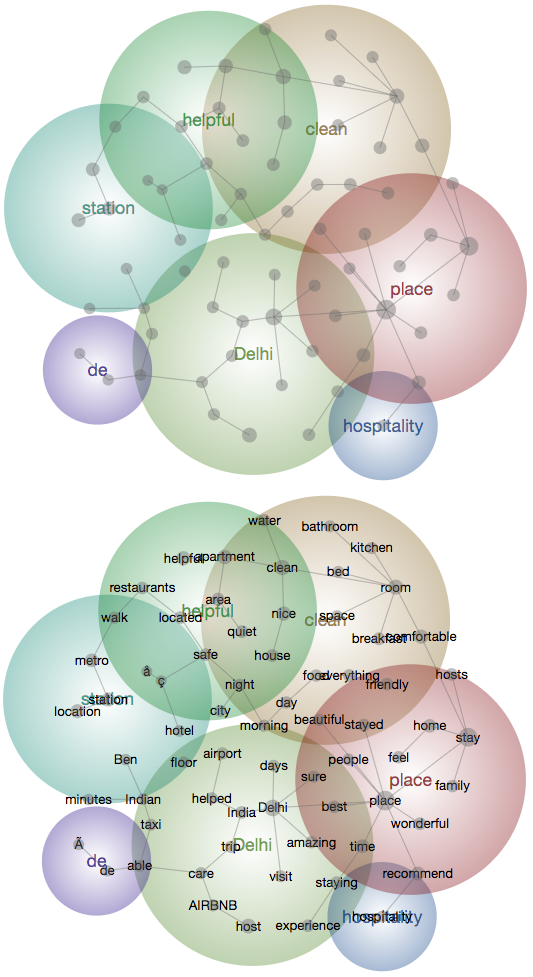
\includegraphics[scale=0.8]{figure6.png} 
\caption{Leximancer analysis of 13,021 reviews of Airbnb hosts in Delhi. Data Mined on 13 July 2018.}
\end{figure}

Some of the words that occur most frequently and are favourable include ‘friendly’, ‘located’, ‘home’, ‘safe’, ‘comfortable’ and ‘kitchen’ (Figure 3). Table 3 in the Appendix gives a comprehensive list of the most frequently occurring words. The likelihood percentage reveals the probability of a word being favourable or unfavourable. For example, reviews that have the word ‘friendly’ have an 89\% likelihood of being favourable. The analysis shows that only 4\% of the total reviews have an unfavourable sentiment.\\

We find that several features and amenities that are invaluable to the consumer are not accommodated in government regulations. For example, the government prohibits B\&Bs from building kitchens and yet ‘kitchen’ appears to be a sought-after feature in Airbnbs. Data mining of Airbnbs in Delhi reveals that out of 453 times that kitchen is mentioned by a guest, its written in a favourable context 427 of those times. That means that almost 95\%  \footnote {Though the data suggests that 95\% of all guests write about kitchens in a positive context, it should be noted that the likelihood of this data being accurate, i.e., of 95\% reviews being desirable, is only 46\%.} of all guests who reviewed the kitchen did so in a favourable context.\\

\subsection{Contrasting the Rules Under the City Taxi Scheme (Delhi) with the Service Requirements Under Uber}
All taxis in Delhi are regulated under the City Taxi Scheme 2015, which merged the Radio Taxi Scheme 2006 and the Economy Radio Taxi Scheme 2010. The Scheme falls under sections 93, 95 and 96 of the Motor Vehicle Act, 1988, and is applicable to all taxi service providers, including an aggregator of taxis. Hereunder, we contrast the specifications under the Scheme with the requirements that service providers need to meet on Uber.\\

\subsubsection{Operational Requirements}
A Group category licensee, under the City Taxi Scheme, requires a web portal with details of its ownership, address, fare structure, services offered and ‘contact details of a duly appointed grievance redressal officer’. The licensee, in both categories, needs to ensure that each taxi is fitted with a temperature control device and a working electronic digital fare metre. A liquid crystal display panel visible from both the front and rear is required to be installed on the roof of the taxi, to communicate whether it is available or not. \\ 

Every taxi also needs to make the photograph of the driver, licence number and registration details of the car visible to the passenger. Other requirements include fitting the taxi with a global positioning system (GPS) and general packet radio service-based tracking device that shows the path traversed and the total distance covered. Finally, the taxi must also have a feedback register that is accessible to passengers at all times.\\

As opposed to this, Uber has select vehicle requirements, such as the capacity to carry four passengers, have four doors and be 15 years old or newer and without missing pieces or cosmetic damages.\\

The app makes redundant some of the conditions under the Scheme such as the requirement to show a the availability of a cab and the need to have a metre or a feedback register. The rating system, for example, functions as a useful proxy to determine the driver’s behaviour with passengers. The app also has an inbuilt GPS system for directions and lists the details of the fare, driver, their photograph, rating, number of past rides and phone number.\\

Before anyone is brought onboard, Uber verifies a set of government documents, such as driving licence, police verification, registration certificate, vehicle insurance and tourist permit.\\

\subsubsection{Ease of Entry and Exit}
The City Taxi Scheme lays out the different requirements for an ‘individual’, who owns a single taxi, or a ‘Group’ that requires a minimum fleet of 200 taxis. \\

Uber, on the other hand, allows for all different variations of owner-driver arrangements. It provides three options to a driver who want to join the app: ‘driver cum owner’, ‘driver under partner’ (driving a vehicle owned by a non-driving person), or as a ‘non-driving partner’ (one who does not drive but owns a vehicle and manages at least one driver).\\

By defining a driver in this way, Uber expands entry in two ways: first, it includes one who does not own a vehicle, and second, it removes capital restrictions for a non-driving partner by allowing anybody with more than one taxi to join the platform. By accommodating all kinds of suppliers under one app, it increases the market size and, therefore, resolves some of the ‘matching’ challenges the industry previously faced. \\

The different ways of associating with the platform and the relatively easier operational mechanisms facilitate market entry for individuals or entrepreneurs who own a fleet of cabs. It allows those who do not own vehicles to lease them through its collaboration with Xchange Leasing India Private Limited. It leases vehicles to Uber partners for up to 60 months, increasing access for those who lack funds to own a vehicle. \\

Finally, Uber allows easy exit from the app and provides drivers with the flexibility to switch to a different firm, aggregator or otherwise, whenever they wish. The flexible nature of working hours allows drivers to join the platform part-time and earn additional income.\\
\subsubsection{Driver Profile}
The City Taxi Scheme mentions that the drivers must have adequate knowledge of city roads, must have completed middle school (have passed at least eighth grade) and must be of good moral character. The driver on duty has to be in a uniform, either as approved by the department or the company. The regulation puts the onus on the licensee (who owns a fleet) to ensure the quality of drivers and their conduct with passengers. The licensee has to ensure that the driver is reliable, trustworthy and safe. Finally, the licensee is required to conduct training sessions for the drivers, to ensure ‘passenger etiquette’ and safe driving skills, at least once a year. \\

To ensure its drivers are trained, Uber makes use of in-app videos, to guide drivers on how they must behave with riders. Further, drivers receive ‘in-person support’ at Uber greenlight hub (a support centre based in the National Capital Region, to address the queries of drivers), on things such as learning how to install the app, setting up an account and dealing with other queries. Uber attempts to improve their user interface constantly to enhance the experiences of both riders and drivers. \\

Uber also puts in place certain ‘community guidelines’ (that cover areas such as discriminatory behaviour, fraud, safety and quality) to ensure a ‘respectful and safe environment’ for the users. This helps guide the behaviour of drivers (as well as riders) and assists them in maintaining a higher rating. These guidelines also explicitly mention that the driver or rider may lose access to the app (temporarily blocked or deactivated) if they fail to comply with the terms. After a period of warning, if the rating of a driver continues to fall below a particular threshold or the driver is involved in a certain number of offences, they may be penalised. Since such an action limits the earning of a driver, it helps to establish checks against the dishonest behaviour. \\

\subsubsection{Fare Structure}
Under the City Taxi Scheme, a licensee is required to charge the fare prescribed by the department of transport. The licensee can also include waiting charges and night charges as approved by the department of transport. As opposed to this, Uber follows dynamic pricing, as determined by its algorithm, based on the supply and demand (and, in some instances, estimated traffic). In situations when demand exceeds supply, there is a surge in the prices to incentivise the drivers to go where there is high demand. As a result, it tries to ensure that supply meets demand to maintain an overall efficient outcome. Once the balance is brought out, prices go back to normal.  \\

In order to be fair, Uber attempts to be completely transparent about this dynamic pricing model and its working. The riders are informed about the surge in prices in case they wish to switch to cheaper alternatives for transport. This mechanism plays an important role in reducing the number of unfulfilled requests and matching the demand and supply, especially during peak travel hours.\\
\subsubsection{Suspension of Licence}
According to the City Taxi Scheme, if the licensee fails to comply with the terms and conditions mentioned under the Scheme, the licencing authority may suspend their licence for a particular period of time or cancel it. \\

In the case of Uber, instead of the decision on the suspension of licence being taken by a particular licencing authority, it is based on the ratings given collectively by the riders who experience the service. Not only this, the rating system increases the accessibility of records and the influence of timelines since the entire history of a driver can be tracked.\\

While many of the specifications laid down under the City Taxi Scheme are made with the intention of protecting the consumers and ensuring their safety, they often become difficult to enforce and implement. These specifications also require regular crackdowns and inspections. Furthermore, rules such as ensuring that the driver is of a ‘good moral character’ and has ‘adequate knowledge of the roads’ are riddled with ambiguity and are difficult to check or enforce. On the other hand, through the use of its app-based technology, matching algorithm, feedback mechanisms and a set of incentives, Uber has managed to provide many of these facilities with ease.\\

\section{Rethinking the Regulatory Approach for \\Aggregators}
The disruption caused by aggregators has intensified the debate on the kind of regulation appropriate for them. A key distinction between a traditional business and that of an aggregators’ is that the former has full control of almost every aspect of the goods and services they provide and can thereby devise in-house policies to govern their actions. On the other hand, aggregators identify themselves as ‘matchmakers’ and not service providers. By extension, they don't hold themselves liable and only claim to mediate grievances between aggrieved participants. 
          
             Two kinds of regulatory responses can be taken towards aggregators:         
                    \begin{enumerate}
                      \item  Reactionary, status-quo sympathetic or product based;
                      \item Anticipatory, accommodative or principles-based.
                    \end{enumerate}
                    
                 Under a reactionary, status-quo sympathetic or product-based regulatory framework, aggregators would be defined and treated similarly to traditional enterprises and all regulations imposed on the latter will have to be met by the former. \\
Many traditional businesses oppose the recent growth of aggregators on the grounds that they continue to face the regulatory burdens that these new entrants are evading \parencite{koopman2014sharing}. This includes licencing requirements, permits, taxation and administrative clearances amongst other things. \\

For instance, listings on platforms such as Airbnb do not have to meet the onerous regulations governing licensed hotels in India. Over 42 licences are required to start and operate a hotel in the organised sector in India. Moreover, five-star hotels pay 38\% of their room revenue as taxes. The Hotel and Restaurant Association of Western India uses this to argue for a uniform and a level playing field for all those in the hospitality sector \parencite{Chaturvedinews}.\\

Similarly, Meru Cabs, a taxi cab service based in Mumbai, accused Uber of following predatory pricing in order to increase their market share. The chief executive officer of Meru Cabs, Nilesh Sangoi, reasons that the huge subsidy given to drivers and impractical discounts to customers offered by Uber has distorted the taxi service market \cite{Kalra2017}.\\

However, once Airbnb listings begin to comply with all the regulations governing hotels or B\&Bs, they will cease to be attractive. Once all regulations that apply to taxicab companies apply to Uber, it will cease to be Uber.\\

While regulations are necessary in the face of the exploitation of consumers and information asymmetries, they generally fail to be dynamic and respond to changes in the market by constraining businesses and innovation. Such regulations, although intended to protect consumers by preventing worst-case scenarios, often end up preventing the best-case scenarios from ever surfacing \cite{koopman2014sharing} . Excessive regulations also result in business harassment by inspectors who demand bribes or favours in exchange of favourable reports. Further, since state capacity is limited, having extensive areas of intervention leads to the government spreading itself thin.\\

In thinking through a regulatory approach to govern aggregators within sector-specific regulations, it is essential to recall that the aggregator business model makes it profitable to reduce friction between the transacting parties, solidify trust and facilitate economic transactions. By treating both service providers and buyers as customers of the platform, aggregators encourage accountability on both sides. Instead of emphasising guarantees and warranties, platforms create mechanisms that incentivise buyers and sellers to reveal necessary information and act in mutual interest. Moreover, they enable users to set standards for safety and quality collectively. \\

The limitations in adopting a status quoist or reactionary approach for regulating aggregators nudges us to explore the merits of a principles-based and accommodative approach. A principles-based regulation does not need to be revised with every change in the service offering. Rather, it entails instituting guidelines that have a high level of generality. Irrespective of how the market changes, it works by creating overarching requirements as opposed to binding rules.\\

\section{Conclusion}
Most regulations that currently apply to service providers ignore the idea that every current market failure is an opportunity, incentivising entrepreneurial efforts to tackle it \cite{thierer2015internet}. \\
The growth of aggregators has transformed the delivery and nature of the services sector, particularly in hospitality and transportation. In a constantly evolving and changing market, regulations in India are failing to keep up with the dynamism of the market. \\

The ‘regulatory lag’ in developing specification-based regulations raises questions on the applicability of the existing framework to the new ways of service delivery. When new ways of regulation have not emerged and old ways become obsolete, the vacuum creates an opportunity for firms to self-regulate in response to consumer needs and concerns. The purpose of our research is to describe the phenomenon of self- and third-party regulation emerging with the growth of aggregators such as Uber, Airbnb and Zomato, and explain how it resolves some of the information problems. \\

While aggregators in India have been accused of ‘regulatory arbitrage’ and considered rule-breakers, there is insufficient research on the unconventional ways in which they are meeting these rules and making new ones. Using existing literature, a thorough analysis of their websites and data mining, we have shown the type of market that the aggregators have opened up for both consumers and service providers. In the process of growing their business, they have developed several trust-building mechanisms and sets of standards (both in the form of laying down guidelines and user feedback) that have inadvertently started tackling the issues of market failure and consumer protection. \\

Our contrast of consumer preferences to the language adopted by regulations points at how conventional rule making in India is, in some instances, at odds with customer needs and preferences. Our research shows that the mechanisms adopted by aggregators are helping meet these needs and preferences differently: by defining standards broadly and creating incentives to increase consumer satisfaction. Not only this, these standards are also constantly being revised.\\

In response to the existing challenge of regulating aggregators, we highlight how the solution may lie in moving towards a principles-based approach. Such an approach can be at once accommodative of innovations and changes in the market, without compromising on the underlying objective of protecting consumers and dealing with market failures. Further, it would help free up state capacity, by encouraging regulatory retreat in areas where it may no longer be required and by doing away with obsolete laws. This, in turn, is likely to reduce the regulatory burden on firms while making sure that no leniency is granted with respect to consumer protection. \\

While our paper suggests a need to rethink existing regulations through a brief analysis of the new methods introduced by aggregators and the gaps in current regulations, further research is required to understand the basis for drawing new frameworks. The answer could lie in understanding the red lines of standards that all enterprises in the sector ought to meet, irrespective of their business model.\\

               
         
% Print Bibliography

	\printbibliography[title={Bibliography}]
	\newpage

%Appendix
  \section*{Appendix 4: Amenities Provided by Airbnbs}
             \addcontentsline{toc}{section}{Appendix 4: FIX}

\begin{longtable}{p{5.5cm}p{2cm}p{5.5cm}p{2cm}}
\caption{Number of Airbnbs providing Each Amenity in Delhi. Data mined on 13 July 2018} \\
Amenity & No. of Airbnbs & Amenity & No. of Airbnbs \\
\midrule
\endfirsthead
Amenity & No. of Airbnbs & Amenity & No. of Airbnbs \\
\midrule
\endhead
\endfoot
\endlastfoot

Air-conditioning & 301 & Hot tub & 7 \\
Baby bath & 2 & Hot water & 247 \\
Babysitter recommendations & 2 & Indoor fireplace & 4 \\
Bathtub & 4 & Iron & 238 \\
Barbecue grill & 21 & Kitchen & 264 \\
Bed linens & 144 & Lake access & 1 \\
Breakfast & 129 & Laptop-friendly workspace & 265 \\
Building staff & 103 & Lock on the bedroom door & 152 \\
Cable TV & 187 & Lockbox & 2 \\
Carbon monoxide detector & 47 & Long-term stays allowed & 187 \\
Changing table & 2 & Luggage dropoff allowed & 156 \\
Children's books and toys & 23 & Microwave & 124 \\
Children's dinnerware & 2 & Outlet covers & 1 \\
Cleaning before checkout & 13 & Oven & 49 \\
Coffee maker & 60 & Pack 'n Play/travel crib & 1 \\
Cooking basics & 117 & Paid parking off premises & 31 \\
Crib & 2 & Paid parking on premises & 10 \\
Dishes and silverware & 113 & Patio or balcony & 84 \\
Dishwasher & 9 & Pocket Wifi & 13 \\
Dryer & 132 & Pool & 7 \\
Elevator & 78 & Private entrance & 131 \\
Essentials & 312 & Private living room & 21 \\
Ethernet connection & 14 & Stair gates & 10 \\
Electric vehicle charger & 7 & Stove & 113 \\
Extra pillows and blankets & 108 & Table corner guards & 1 \\
Fire extinguisher & 148 & TV & 235 \\
Fireplace guards & 1 & Washer & 204 \\
First aid kit & 215 & Waterfront & 8 \\
Free parking on premises & 180 & Wifi & 307 \\
Free street parking & 150 & Window guards & 8 \\
Game console & 2 & Refrigerator & 153 \\
Garden or backyard & 42 & Room-darkening shades & 17 \\
Gym & 21 & Shampoo & 260 \\
Hairdryer & 199 & Single level home & 32 \\
Hangers & 276 & Ski in/Ski out & 2 \\
Heating & 202 & Smart lock & 1 \\
High chair & 13 & Smoke detector & 66 \\
Host greets you & 123 \\

\end{longtable}

\newpage





%APPENDIX 2

 \section*{Appendix 4: Sentiment Analysis for Reviews of all Airbnbs}
             \addcontentsline{toc}{section}{Appendix 4: FIX}

\footnotesize
\begin{longtable}{p{2cm}p{2cm}p{1cm}p{1.6cm}p{2.4cm}p{1.9cm}p{1cm}p{2cm}}
\caption{Sentiment Analysis for Reviews of all Airbnbs in Delhi. Data mined on 13 July 2018} \\
Concept & Word & Count & Likelihood Percent & Concept & Word & Count & Likelihood Percent \\
\midrule
\endfirsthead
Concept & Word & Count & Likelihood Percent & Concept & Word & Count & Likelihood Percent \\
\midrule
\endhead
\endfoot
\endlastfoot

favourable & wonderful & 1289 & 91\% & unfavourable & night & 60 & 5\% \\
favourable & nice & 2428 & 91\% & unfavourable & water & 63 & 5\% \\
favourable & helpful & 2480 & 90\% & unfavourable & helped & 44 & 5\% \\
favourable & beautiful & 937 & 89\% & unfavourable & hotel & 28 & 5\% \\
favourable & friendly & 1322 & 89\% & unfavourable & taxi & 33 & 4\% \\
favourable & best & 1149 & 87\% & unfavourable & people & 45 & 4\% \\
favourable & location & 1764 & 69\% & unfavourable & sure & 41 & 4\% \\
favourable & hosts & 1001 & 69\% & unfavourable & floor & 18 & 4\% \\
favourable & host & 2636 & 69\% & unfavourable & day & 47 & 4\% \\
favourable & restaurants & 831 & 67\% & unfavourable & airport & 44 & 4\% \\
favourable & food & 810 & 64\% & unfavourable & able & 16 & 4\% \\
favourable & breakfast & 1078 & 63\% & unfavourable & trip & 34 & 4\% \\
favourable & experience & 1011 & 63\% & unfavourable & bathroom & 26 & 3\% \\
favourable & located & 760 & 62\% & unfavourable & bed & 24 & 3\% \\
favourable & area & 960 & 60\% & unfavourable & experience & 54 & 3\% \\
favourable & quiet & 778 & 60\% & unfavourable & days & 26 & 3\% \\
favourable & clean & 2119 & 59\% & unfavourable & everything & 45 & 3\% \\
favourable & apartment & 1744 & 58\% & unfavourable & city & 29 & 3\% \\
favourable & metro & 1078 & 58\% & unfavourable & room & 105 & 3\% \\
favourable & family & 835 & 58\% & unfavourable & morning & 29 & 3\% \\
favourable & hospitality & 476 & 58\% & unfavourable & area & 47 & 3\% \\
favourable & place & 4776 & 57\% & unfavourable & location & 74 & 3\% \\
favourable & station & 1184 & 57\% & unfavourable & stayed & 40 & 3\% \\
favourable & city & 549 & 57\% & unfavourable & kitchen & 26 & 3\% \\
favourable & stay & 4374 & 57\% & unfavourable & apartment & 83 & 3\% \\
favourable & helped & 544 & 56\% & unfavourable & care & 24 & 3\% \\
favourable & space & 417 & 56\% & unfavourable & time & 71 & 3\% \\
favourable & time & 1438 & 56\% & unfavourable & station & 54 & 3\% \\
favourable & comfortable & 1479 & 56\% & unfavourable & nice & 69 & 3\% \\
favourable & house & 882 & 56\% & unfavourable & metro & 45 & 2\% \\
favourable & people & 581 & 55\% & unfavourable & house & 38 & 2\% \\
favourable & safe & 694 & 55\% & unfavourable & best & 31 & 2\% \\
favourable & walk & 452 & 54\% & unfavourable & host & 89 & 2\% \\
favourable & everything & 784 & 54\% & unfavourable & helpful & 60 & 2\% \\
favourable & stayed & 742 & 53\% & unfavourable & walk & 18 & 2\% \\
favourable & bathroom & 400 & 53\% & unfavourable & comfortable & 57 & 2\% \\
favourable & morning & 509 & 52\% & unfavourable & feel & 25 & 2\% \\
favourable & home & 1220 & 52\% & unfavourable & place & 172 & 2\% \\
favourable & feel & 626 & 52\% & unfavourable & amazing & 25 & 2\% \\
favourable & room & 1822 & 52\% & unfavourable & restaurants & 24 & 2\% \\
favourable & airport & 598 & 51\% & unfavourable & safe & 24 & 2\% \\
favourable & day & 621 & 51\% & unfavourable & food & 24 & 2\% \\
favourable & amazing & 644 & 50\% & unfavourable & breakfast & 32 & 2\% \\
favourable & staying & 657 & 49\% & unfavourable & stay & 143 & 2\% \\
favourable & care & 424 & 49\% & unfavourable & hospitality & 15 & 2\% \\
favourable & night & 551 & 48\% & unfavourable & recommend & 55 & 2\% \\
favourable & bed & 337 & 48\% & unfavourable & family & 25 & 2\% \\
favourable & water & 575 & 47\% & unfavourable & hosts & 25 & 2\% \\
favourable & visit & 435 & 47\% & unfavourable & home & 39 & 2\% \\
favourable & kitchen & 427 & 46\% & unfavourable & friendly & 24 & 2\% \\
favourable & trip & 422 & 46\% & unfavourable & beautiful & 16 & 2\% \\
favourable & sure & 442 & 45\% & unfavourable & minutes & 5 & 2\% \\
favourable & recommend & 1291 & 41\% & unfavourable & clean & 54 & 1\% \\
favourable & days & 302 & 39\% & unfavourable & located & 18 & 1\% \\
favourable & floor & 156 & 35\% & unfavourable & visit & 13 & 1\% \\
favourable & hotel & 205 & 33\% & unfavourable & de & 3 & 1\% \\
favourable & taxi & 244 & 32\% & unfavourable & quiet & 17 & 1\% \\
favourable & able & 72 & 17\% & unfavourable & space & 9 & 1\% \\
favourable & minutes & 50 & 15\% & unfavourable & wonderful & 15 & 1\% \\
 &  &  &  & unfavourable & staying & 14 & 1\% \\

\end{longtable}
\normalsize



	     
                    \end{document}